% Modelo de Trabalho Acadêmico da UNESP de Guaratinguetá v-1.0
% Copyright 2017 by Eduardo Rohde Eras
%
% This program is free software: you can redistribute it and/or modify
% it under the terms of the GNU General Public License as published by
% the Free Software Foundation, either version 3 of the License, or
% (at your option) any later version.
%
% This program is distributed in the hope that it will be useful,
% but WITHOUT ANY WARRANTY; without even the implied warranty of
% MERCHANTABILITY or FITNESS FOR A PARTICULAR PURPOSE.  See the
% GNU General Public License for more details.
%
% You should have received a copy of the GNU General Public License
% along with this program.  If not, see <http://www.gnu.org/licenses/>.

%----------------------------------------------------------------------------------------%
% C L A S S E   D O   D O C U M E N T O
%----------------------------------------------------------------------------------------%

\documentclass[
  %----------------------------------------------------------------------------------------%
  %Opções da classe 'memoir'
  %----------------------------------------------------------------------------------------%
  12pt,		% Tamanho da Fonte.
  a4paper,	% Tamanho da página.
  openright,% Capítulos começam em páginas ímpares (insere uma página vazia se necessário).
  oneside,	% Para impressão em frente e verso utilizar twoside.
  %----------------------------------------------------------------------------------------%
  %Opções da classe 'abntex2'
  %----------------------------------------------------------------------------------------%
  chapter=TITLE,		%Títulos de capítulos convertidos em letras maiúsculas.
  section=TITLE,		%Títulos de seções convertidos em letras maiúsculas.
  %----------------------------------------------------------------------------------------%
  %Opções da classe 'babel'
  %----------------------------------------------------------------------------------------%
  english,	%Idioma adicional para hifenização.
  french,	%Idioma adicional para hifenização.
  spanish,	%Idioma adicional para hifenização.
  brazil	%Idioma principal do documento.
  %----------------------------------------------------------------------------------------%
]{abntex2}

%----------------------------------------------------------------------------------------%
% P A C O T E S
%
% Insira aqui os pacotes que for utilizar em seu documento. Para saber quais pacotes o
% template já está utilizando, confira o arquivo "pacoteBasico.sty".
%----------------------------------------------------------------------------------------%
    
    \usepackage{pacoteBasico}   %Pacote Básico de formatação no padrão da UNESP/FEG
    \usepackage{color}		    %Controle das cores.
    \usepackage{graphicx}	    %Inclusão de gráficos.
    \usepackage{lipsum}		    %Para geração de 'Dummy Text'.
    
%----------------------------------------------------------------------------------------%
% I N F O R M A Ç Õ E S   B Á S I C A S   S O B R E   O   T R A B A L H O
%
% Defina aqui as informações pertinentes ao trabalho.
%----------------------------------------------------------------------------------------%

    %----------------------------------------------------------------------------------------%
    % D A D O S   P E S S O A I S
    %----------------------------------------------------------------------------------------%
    
    %Nome completo do autor do presente Trabalho de Graduação:
    \newcommand{\nomeDoAutor}{
    Matheus Cerqueira de Jesus
    }
    
    %Nome do curso em que o autor está se graduando:
    \newcommand{\nomeDoCurso}{
    Engenharia Elétrica
    }
    
    %----------------------------------------------------------------------------------------%
    % D A D O S   S O B R E   O   T R A B A L H O
    %----------------------------------------------------------------------------------------%
    
    %Título do presente trabalho:
    \newcommand{\tituloDoTrabalho}{
    Técnicas de \textit{Machine Learning} para estimar a correlação de queimadas em Cuiabá nas doenças respiratórias.
    }
    
    % Subtítulo do presente trabalho, se houver:
    % \newcommand{\subtituloDoTrabalho}{
    
    % }
    
    %Mês da entrega do trabalho
    \newcommand{\mesDeEntrega}{
    Janeiro
    }
    
    %Ano da entrega do trabalho
    \newcommand{\anoDeEntrega}{
    2023
    }
    
    %----------------------------------------------------------------------------------------%
    % D A D O S   D O S   O R I E N T A D O R E S,   B A N C A   E   C O O R D E N A D O R
    %----------------------------------------------------------------------------------------%
    
    %Nome do orientador do presente trabalho:
    \newcommand{\nomeDoOrientador}{
    Paloma Maria Silva Rocha Rizol
    }
    
    %Título do orientador:
    \newcommand{\tituloDoOrientador}{
    Profº Dr.
    }
    
    %Nome do coorientador do presente trabalho:
    \newcommand{\NomeDoCoorientador}{
    Taynara de Oliveira Castellões
    }
    
    %Título do coorientador:
    \newcommand{\tituloDoCoorientador}{
    Mestranda
    }
    
    %Nome do Coordenador do Curso:
    \newcommand{\nomeDoCoordenador}{
    Nome Completo do Coordenador
    }
    
    %Título do coordenador do Curso:
    \newcommand{\tituloDoCoordenador}{
    Profº Dr.
    }
    
    %Nome do Membro Interno da Banca:
    \newcommand{\nomeDoMembroInterno}{
    Nome Completo do Membro Interno
    }
    
    %Título do Membro Interno da Banca:
    \newcommand{\tituloDoMembroInterno}{
    Profº Dr.
    }
    
    %Nome do membro Externo da banca:
    \newcommand{\nomeDoMembroExterno}{
    Nome Completo do Membro Externo
    }
    
    %Título do Membro Externo da Banca:
    \newcommand{\tituloDoMembroExterno}{
    Profº Dr.
    }
    
    %----------------------------------------------------------------------------------------%
    % D A D O S   D A   I N S T I T U I Ç Ã O
    %----------------------------------------------------------------------------------------%
    
    %Nome da Universidade
    \newcommand{\nomeDaUniversidade}{
    Universidade Estadual Paulista "Júlio de Mesquita Filho"
    }
    
    %Nome da Cidade
    \newcommand{\nomeDaCidade}{
    Guaratinguetá
    }

%----------------------------------------------------------------------------------------%
% I N Í C I O   D O   D O C U M E N T O - P R É   T E X T U A L
%----------------------------------------------------------------------------------------%
\begin{document}
    
    \imprimircapa
    \imprimirfolhaderosto
    
    %------------------------------------------------------------------------------------%
    % F O L H A   D E   A P R O V A Ç Ã O
    %
    % OBRIGATÓRIO. Este é o modelo de folha de aprovação que deve ser digitalizada após as
    % assinaturas da banca. Utilize um software de edição de PDF para substituição posterior
    % dessa folha. Se possível, utilize um recurso de assinatura digital fornecido pela
    % ferramenta de edição de PDF, evitando assim a digitalização da folha toda.
    %------------------------------------------------------------------------------------%
    \begin{folhadeaprovacao}
        \begin{center}
        
        {\sffamily
            \bfseries{
                \Large{
                    UNIVERSIDADE ESTADUAL PAULISTA\par
                    "JÚLIO DE MESQUITA FILHO"\par
                }
            }
            CAMPUS DE GUARATINGUETÁ
        }
        
        \vspace*{3cm}
                
        \normalsize{\textbf{\MakeUppercase\nomeDoAutor}}
        
        \vspace*{1cm}
        
       % {\setstretch{1.0}
        \begin{framed}
            ESTE TRABALHO DE GRADUAÇÃO FOI JULGADO ADEQUADO COMO PARTE DO REQUISITO PARA A OBTENÇÃO DO DIPLOMA DE \textbf{"GRADUANDO EM {\MakeUppercase\nomeDoCurso}"}
            \par
            \vspace*{1cm}
            APROVADO EM SUA FORMA FINAL PELO CONSELHO DE CURSO DE GRADUAÇÃO EM {\MakeUppercase\nomeDoCurso}
            \par
            \vspace*{1cm}
            \begin{flushright}
            \tituloDoCoordenador {\MakeUppercase\nomeDoCoordenador}
            \par
            Coordenador
            \end{flushright}
       \end{framed}
      % }
       
       \begin{flushleft}
            \textbf{BANCA EXAMINADORA:}
       \end{flushleft}
       
       \assinatura{\small \tituloDoOrientador \nomeDoOrientador \par Orientador/UNESP-FEG}
       \assinatura{\small \tituloDoMembroInterno \nomeDoMembroInterno \par UNESP-FEG}
       \assinatura{\small \tituloDoMembroExterno \nomeDoMembroExterno \par Membro Externo}
       
       \vfill
       \mesDeEntrega, \anoDeEntrega
        
        \end{center}
    \end{folhadeaprovacao}
    
    %------------------------------------------------------------------------------------%
    % D A D O S   C U R R I C U L A R E S
    % 
    % OBRIGATÓRIO PARA PÓS-GRADUAÇÃO.
    % Inserir a data inicial e final de cada formação acadêmica. Para os alunos que não
    % precisarem de uma folha de dados curriculares em seu trabalho, basta apagar todo 
    % o código dessa seção.
    %------------------------------------------------------------------------------------%
    
    \begin{center}
        \normalsize{\textbf{\MakeUppercase{Dados Curriculares}}} \par
        \vspace*{1cm}
        \normalsize{\textbf{\MakeUppercase\nomeDoAutor}} \par
        \vspace*{1cm}
        
        \begin{tabular}{ l p{7cm} }
            \textbf{\MakeUppercase{Nascimento}} & Data - Cidade / Sigla do Estado \\
            \\
            \textbf{\MakeUppercase{Filiação}} & Antonio Sergio de Jesus \\
            & Maria do Socorro Cerqueira de Jesus \\
            \\
            \textbf{\MakeUppercase{Ano Inicial / Ano Final}} & Formação acadêmica ou Complementar (nome do curso e titulação) \\
            & Instituição de Ensino \\
            \\
            \textbf{\MakeUppercase{Ano Inicial / Ano Final}} & Formação acadêmica ou Complementar (nome do curso e titulação) \\
            & Instituição de Ensino \\
            \\
            \textbf{\MakeUppercase{Ano Inicial / Ano Final}} & Formação acadêmica ou Complementar (nome do curso e titulação) \\
            & Instituição de Ensino \\
        \end{tabular}
    \end{center}
    \newpage
    
    %------------------------------------------------------------------------------------%
    % D E D I C A T Ó R I A
    %
    % OPCIONAL. Se não for utilizar uma dedicatória, basta apagar todo o código dessa seção.
    %------------------------------------------------------------------------------------%
    
    \begin{dedicatoria}
        \vspace*{\fill}
        \begin{flushright}
            Sua dedicatoria deve ser digitada aqui.
        \end{flushright}
        \vspace*{1cm}
    \end{dedicatoria}

    %------------------------------------------------------------------------------------%
    % A G R A D E C I M E N T O S
    %
    % OPCIONAL. Citar as pessoas, instituição, agência de fomento, entre outros que contribuíram
    % de maneira relevante à elaboração do trabalho e na vida acadêmica.
    % Se não for utilizar os agradecimentos, basta apagar todo o código dessa seção.
    %------------------------------------------------------------------------------------%
    \begin{agradecimentos}
    
        Esse é um espaço reservado para os agradecimentos. Uma nota de rodapé\footnote{Essa é uma nota de rodapé} pode ser inserida desta forma para indicar alguma URL\footnote{\url{http:\\www.url.com.br}} que referencia o alvo de seu agradecimento.
    
    \end{agradecimentos}
    
    %------------------------------------------------------------------------------------%
    % F O M E N T O
    %
    % OBRIGATÓRIO PARA ALUNO BOLSISTA. Esta página contém informações sobre o financiamento
    % recebido para o desenvolvimento da tese/dissertação. Utilize o(s) nome(s) da(s) 
    % instituição(ões) que forneceu(ram) o auxílio financeiro para seu trabalho. Se não
    % for utilizar o fomento em seu trabalho, basta apagar todo o código dessa seção.
    %------------------------------------------------------------------------------------%
    % \vspace*{\fill}
    % \begin{flushleft}
    %     Este trabalho contou com o apoio da(s) seguinte(s) entidade(s):\\
    %     FAPESP - Fundação de Amparo à Pesquisa do Estado de São Paulo\\
    %     CAPES - Coordenação de Aperfeiçoamento de Pessoa de Nível Superior\\
    %     CNPq - Conselho Nacional de Desenvolvimento Científico e Tecnológico\\
    %     SIGQ - Sigla de Uma Instituição Genérica Qualquer
    % \end{flushleft}
    % \newpage
    
    %------------------------------------------------------------------------------------%
    % E P Í G R A F E
    %
    % OPCIONAL. Texto em que o autor apresenta uma citação, seguida de indicação de autoria.
    % Se não for utilizar uma epígrafe, basta apagar todo o código dessa seção.
    %------------------------------------------------------------------------------------%
    
    \begin{epigrafe}
        \vspace*{\fill}
    	\begin{flushright}
    		\textit{
        		``Frase, citação, epígrafe.``\\
        		(Autor)
    		}
    	\end{flushright}
    \end{epigrafe}
    
    %------------------------------------------------------------------------------------%
    % R E S U M O   N O   I D I O M A   D O   T E X T O
    %
    % OBRIGATÓRIO. Deve ser redigido em um só parágrafo contendo de 150 a 500 palavras e 
    % ressaltar: objetivo, método, resultados e as principais conclusões.
    % Após o resumo, são listadas palavras-chave relacionadas à temática do trabalho, 
    % separadas entre si por ponto e também finalizadas por ponto.  (NBR 6028, 2003)
    %------------------------------------------------------------------------------------%
    
    \begin{resumo}
    
        \lipsum[1] % Digite seu resumo no lugar deste comando.
        
        \vspace*{0.5cm}
    
        \noindent\textbf{\MakeUppercase{Palavras-Chave: }} palavra-chave. palavra-chave. palavra-chave.
    
    \end{resumo}
    
    %------------------------------------------------------------------------------------%
    % A B S T R A C T :   R E S U M O   N O   I D I O M A   E S T R A N G E I R O
    %
    % OBRIGATÓRIO. Elaborado com as mesmas características do resumo em língua portuguesa.
    % Se redigido em inglês-ABSTRACT, em castelhano-RESUMEN, em francês-RÉSUMÉ.
    % Após o resumo, são listadas palavras-chave relacionadas à temática do trabalho no 
    % idioma escolhido. Se redigido em inglês - KEYWORDS, em espanhol - PALABRAS CLAVES,
    % em francês - MOTS-CLÉS.
    %------------------------------------------------------------------------------------%
    
    \begin{resumo}[Abstract] % Substitua 'Abstract' pela palavra no idioma desejado, caso precise.
    
        \lipsum[1] % Digite seu abstract no lugar deste comando.
        
        \vspace*{0.5cm}
        
        %Subistitua 'Keywords' pela palavra no idioma desejado, caso precise.
        \noindent\textbf{\MakeUppercase{Keywords: }} keyword. keyword. keyword.
    
    \end{resumo}
    
    %------------------------------------------------------------------------------------%
    % L I S T A   D E   I L U S T R A Ç Õ E S
    %
    % OPCIONAL. Quando necessário recomenda-se a elaboração de lista própria para cada tipo
    % de ilustração (figuras, fotografias, organogramas, quadros, etc).(NBR14724, 2011)
    % Se não for utilizar uma Lista de Ilustrações, basta apagar todo o código dessa seção.
    %------------------------------------------------------------------------------------%
    
    \listoffigures*
    \newpage
    
    %------------------------------------------------------------------------------------%
    % L I S T A   D E   T A B E L A S
    %
    % OPCIONAL. Se não for utilizar uma Lista de Tabelas, basta apagar todo o código
    % dessa seção.
    %------------------------------------------------------------------------------------%
    
    \listoftables*
    \newpage
    
    %------------------------------------------------------------------------------------%
    % L I S T A   D E   A B R E V I A T U R A S   E   S I G L A S
    %
    % OPCIONAL. Consiste na relação alfabética das abreviaturas e siglas utilizadas,
    % seguidas das palavras ou expressões correspondentes escritas por extenso.
    % Se não for utilizar uma Lista de Abreviaturas, basta apagar todo o código dessa seção.
    %------------------------------------------------------------------------------------%
    
    \begin{siglas}
        \item[TCC] Trabalho de Conclusão de Curso
        \item[UNESP] Universidade Estadual Paulista
        \item[IA] Inteligência Artificial
    \end{siglas}
    
    %------------------------------------------------------------------------------------%
    % L I S T A   D E   S Í M B O L O S
    %
    % OPCIONAL. Os símbolos devem ser listados de acordo com a ordem apresentada no texto,
    % com seus respectivos significados. Se não for utilizar uma Lista de Símbolos, basta
    % apagar todo o código dessa seção.
    %------------------------------------------------------------------------------------%
    
    \begin{simbolos}
        \item[$\alpha$] Letra Grega Alfa
        \item[$\beta$] Letra grega Beta
        \item[$\gamma$] Letra grega Gama
        \item[$e$] Número de Euler
        \item[R\$] Unidade monetária Brasileira (Real)
    \end{simbolos}
    
    %------------------------------------------------------------------------------------%
    % S U M Á R I O
    %
    % OBRIGATÓRIO. Havendo mais de um volume, cada um deve conter o sumário completo do
    % trabalho (NBR6024; NBR6027, 2012). Não se deve confundir sumário com índice.
    %------------------------------------------------------------------------------------%
    
    \tableofcontents*
    \newpage
    
    %------------------------------------------------------------------------------------%
    %                                                                                    %
    %                           C O R P O   D O   T E X T O                              %
    %                                                                                    %
    %                     Seu trabalho começa a ser digitado aqui.                       %
    %                                                                                    %
    % Início do corpo do texto. A partir desse comando será impresso o número de páginas.%
    %------------------------------------------------------------------------------------%
    
    \textual
    \pagestyle{simple} 
    
    %------------------------------------------------------------------------------------%
    
    \chapter{Introdução}
    Os últimos séculos foram marcados por períodos de intensos desenvolvimentos tecnológicos, sendo impulsionados
    pelas revoluções industriais. As indústrias são responsáveis por produzir a maior
    parte dos produtos essenciais para os seres humanos, bem como o desenvolvimento de novos produtos.
    Para a produção de carros cada vez mais potentes, escalas enormes de alimentos, dispositivos digitais, produtos farmacêuticos
    é necessária a produção de energia para o funcionamento das máquinas das indústrias, automóveis para o transporte de cargas e pessoas,
    e atender as populações das cidades e do campo.

    No entanto, de acordo com a \cite[]{iea} a matriz energética mundial é majoritariamente
    composta por fontes de energia não renováveis e altamente poluentes, como os combustíveis
    fósseis, sendo eles, carvão mineral, petróleo e gás natural. 
    Diante do consumo constante dessas matrizes energéticas os níveis de poluentes na atmosfera
    passaram a aumentar. E com isso a necessidade de realizar estudos para entender a influencia
    desses poluentes na saúde humana.

    Segundo a \cite[]{diretrizes_oms} uma estimativa realizada em 2021 aponta que a cada ano, a exposição
    à poluição atmosférica seja responsável por 7 milhões de mortes prematuras e milhões de anos de vida
    reduzidos de pessoas com uma vida saudável em todo o mundo. Outro agravante relacionado a poluição é o aumento
    temperatura média do planeta que segundo a \cite[]{temperatura_onu} em 2021 a temperatura média do planeta foi de 1,1\degree C acima
    da linha base pré-industrial. Diante dessa situação, \cite[]{pneumonia_temperatura} apontam que as altas e baixas temperaturas
    estão associadas com o aumento da incidência de casos de pneumonia e que as altas variações de temperatura diurnas e entre dias
    podem afetar o funcionamento do sistema respiratório.

    Diante desse contexto, a demanda dos serviços de saúde estão cada vez maiores e situações em que os serviços operam acima da capacidade
    máxima estão cada vez mais frequentes. Conforme apresentado por \cite[]{Health} os sistemas e serviços de saúde necessitam de recursos essenciais
    para atuar, incluindo informações hospitalares, doenças e previsões. No entanto, de acordo com \cite[]{forcasting_health}, os hospitais, serviços de saúde
    e fornecedores geralmente não estão adequadamente informados quando entram em uma situação de demanda acima do normal.
    
    Este trabalho, reuniu dados e informações diárias relacionados a qualidade do ar, temperatura ambiente e internações ocorridas em hospitais
    de Cuiabá no estado do Mato Grosso entre 01/01/2013 e 31/12/2018 para treinar modelos de \textit{Machine Learning} e redes neurais afim de predizer
    o número de internações nos dias subsequentes a uma determinada data, utilizando como dados de entradas os valores de qualidade do ar
    e temperatura. Os resultados dos diferentes modelos foram comparados, observando principalmente o raiz do erro quadrático médio(RMSE).
    
    \section{objetivos}
    Este trabalho tem como objetivo utilizar técnicas de \textit{Machine Learning} e redes neurais artificiais a fim de predizer 
    internações hospitalares de pacientes com doenças respiratórias
    causadas por puluições atmosféricas.
    \section{justificativas}
    Na palaforma Scopus foram realizadas três pesquisas a fim de verificar o contexto de trabalhos
    realizados na academia com temas semelhantes aos deste trabalho, conforme apresentado na Tabela \ref*{tabela scopus}.
    Nota-se que para a pesquisa com as palavras chave: Machine learning, respiratory diseases e air quality 
    foram publicados somente 66 artigos, isso mostra ser um tema que ainda não foi muito pesquisado, apesar de estar em crescimento.

    Ao adicionar Cuiabá nas palavras chave da busca, não foi retornado nenhum resultado, isso indica que o trabalho realizado é inédito.

    \begin{table}[h]
        \centering
        \caption{Publicações no Scopus}
        \label{tabela scopus}
        \begin{tabular}{ccc}
            \hline
            \multicolumn{1}{|c|}{Pesquisa} & \multicolumn{1}{c|}{Período} & \multicolumn{1}{c|}{Total de publicações}\\
            \hline
            "\textit{Machine Learning}" & 2012 - 2022 & 445203 \\
            "\textit{Machine Learning}" e "Respiratory Diseases" & 2012 - 2022 & 2.264 \\
            "\textit{Machine Learning}" e "Respiratory Diseases"  e "Air Quality" & 2012 - 2022 & 66 \\
            \hline
        \end{tabular}
        \par
        {\small fonte: Scopus (2023)}
    \end{table}

    \section{delimitações da pesquisa}
    Ao decorrer do trabalho foram verificadas algumas limitações responsáveis por restringir o alcance do estudo.
    Os dados utilizados para o treinamento dos modelos de \textit{Machine Learning} e (RNA) possuem 
    colunas com informações sobre a qualidade do ar, temperatura, umidade e internações por doenças respiratórias. Os dados de qualidade
    do ar são estimativas realisadas pelo SISAM para a cidade de Cuiabá-MT, assim considerou-se que todos os habitantes 
    estão submetidos as mesma condições.

    Ao considerar que todas as pessoas estão influênciadas pelas mesmas condições, desconsidera-se 
    as condições de onde essas pessoas vivem e com o que elas trabalham. Por exemplo, uma pessoa que trabalhe em uma marcenaria
    está sobre condições respiratórias piores do que outras pessoas e essa influência não foi levada em conta nos modelos por não possuir dados.

    Os dados de internações representam apenas as internações ocorridas nos hospitais da rede pública (SUS). Dessa forma, todas as internações
    por doenças respiratórias ocorridas na rede particular de hospitais não foram contabilizadas. Ainda, as informações das internações por doenças 
    respiratórias são diagnosticadas pelos médicos e inseridas no sistema SIH/SUS, portanto pode haver algum engano ao ser inserida uma informação
    errada no sistema.

    \section{estrutura do trabalho}

    \chapter{fundamentação teórica}
    Neste capítulo foi escrita uma descrição resumida das ferramentas, técninas e conceitos utilizados
    no desenvolvimento do trabalho.
    \section{python e ciência de dados}
    25/01
    
    Python é uma linguagem de programação de computadores multiparadigma e de código aberto (\textit{open source}), 
    que de acordo com \cite[]{learning_python} é ótimazada para programar de forma produtiva, ler e entender os códigos
    com facilidade e qualidade de software.

    Python é a linguagem mais utilizada do mundo segundo o rank da linguagens de \cite[]{PYPL} ganhando de Java, Java Script e C++. Essa liderança
    explica a extensa comunidade que a linguagem possui, sendo isso uma vantagem para quem utiliza, uma vez que é possível encontrar milhares
    de exemplos de código para uma possível aplicação que alguém precise.
    
    Uma ótima vantagem da linguagem é a íncrivel quantidade de bibliotecas disponibilizadas pela comunidade para as mais variadas aplicações. Isso
    torna o Python uma ótima ferramenta para trabalhar com inteligência artificial, \textit{Machine Learning} e \textit{deep learning}. Algumas das principais
    bibliotecas e \textit{frameworks} utilizadas são Pandas e Numpy para a manipulação de dados, TensorFlow e Scikit Learning para
    a contrução de modelos de \textit{Machine Learning}, como os que serão abordados nos capítulos \ref*{IA} e \ref*{LSTM}.
    
    \section{Inteligência artificial no contexto da saúde}
    \label{IA}
    25/01

    Inteligência artificial tem sido um assunto amplamente abordado pelas pessoas em vídeos, notícias e filmes. Muitos
    acreditam que ela pode ser a solução para todos os problemas existentes na sociedade. No entanto, é importante
    saber o que realmente é inteligência artificial e para o que ela realmente pode ser usada.

    O professor \cite[]{IA_python} define em seu livro inteligência artificial como sendo uma área de estudo dentro ciências da computação
    que possui o objetivo de fazer com que máquinas aprendam a interpretar e resolver problemas de maneira similar
    ao ser humano. Da mesma forma que um ser humano, aprende ao tentar resolver problemas e obter novas informações, uma inteligência artificial
    deve tomar uma ação a medida em que recebe novas informações e aprende a fim de melhorar sua performance.

    Alguns exemplos de inteligência artificial presente no dia a dia de muitas pessoas são as assistentes virtuais
    como a Alexa da Amazon e a Cortana da Microsoft, outro exemplo são as ferramentas de anúncio na internet que aprendem
    com informações sobre os usuários e enviam anúncios de maior interesse. Mas como as IAs, estam relacionadas 
    com a saúde das pessoas e os serviços de assistência médica?
    
    De acordo com Trishan Panch: 
    \vspace{1.5pt}
            \begin{flushright}
                \begin{minipage}{.724\textwidth}
                    {\SingleSpacing\small
                    A Inteligência Artificial e o aprendizado de máquina têm o potencial de ser o catalisador da transformação
dos sistemas de saúde para melhorar a eficiência e a eficácia, criar margem
para a cobertura universal de saúde e melhorar os resultados. \cite[p.1]{IA_health_systems}
                    }
                \end{minipage}
            \end{flushright}
            \vspace{1.5pt}

    Nos sistemas de saúde existem processos que podem utilizar IAs. Dois exemplos são segundo \cite[]{IA_health_systems}
    o diagnóstico de doenças dos pacientes, realizando uma tarefa de classificação, se está ou não com a doença. O outro processo
    se da durante o tratamento, envolvendo predição de uma melhora ou piora no quadro do paciente, monitorando os dados vitais. Algumas das
    aplicações existentes foram apresentadas na tabela \ref*{tabela aplicações IA Med}.

    \begin{table}[h]
        \centering
        \caption{Aplicações de IAs na medicina}
        \label{tabela aplicações IA Med}
        \begin{tabular}{cc}
            \hline
            \multicolumn{1}{|c|}{Diagnóstico} & \multicolumn{1}{c|}{Prognóstico e predição}\\
            \hline
            Analise de imagem: Mamografia & Hospitalização por doença cardíaca\\
            Analise de sinais: Monitoramento intraparto & Risco de acidente cardiovascular\\
            Analise de imagem: identificação da retinopatia diabética& Predição de resultados em câncer colorretal\\
            \hline
        \end{tabular}
        \par
        {\small fonte: Adaptado de \cite[]{IA_health_systems}}
    \end{table}

    Diante disso, é notavel que as IAs podem contribuir para melhorar os serviços de saúde, impactando a vida
    de milhares de pessoas. A seguir serão abordadas algumas técnicas de aprendizado de maquinas utilizadas neste trabalho.
    \subsection{\textit{Machine Learning}}
    26/01


    \subsubsection{\textit{Decision Trees}}
    26/01
    
    Árvores de decisão (\textit{Decision Trees}) são algoritmos de \textit{machine learning} muito versáteis, que podem ser utilizados
    tanto para resolver problemas de classificação quanto de regressão.
    Como o próprio nome diz as \textit{Decision Trees} possuem uma estrutura hierarquia em árvore, contendo o nó raiz (\textit{root node}),
    as ramificações, nós de decisão (\textit{decision nodes}) e as folhas (\textit{leaf nodes}). Uma estrutura simples desse algoritmo
    está apresentada na \ref*{estrutura_decision_tree}.

    \begin{figure}[h]
        \centering
        \caption{Estrutura das árvores de decisão}
        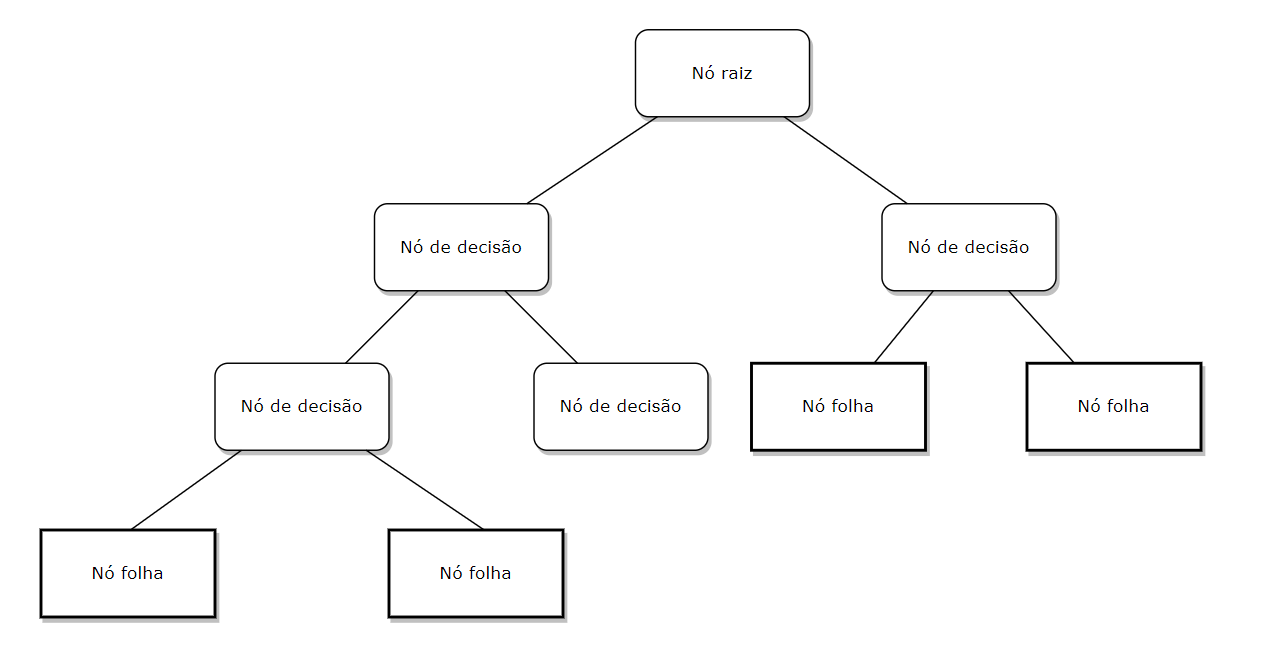
\includegraphics[width=16cm]{../reports/figures/decision_tree_exemple.png}
        \label{estrutura_decision_tree}
        \par
        {\small fonte: Produção do próprio autor.}
    \end{figure}

    O modelo de \textit{Decision Trees} utilizado nesse trabalho realizou uma tarefa de regressão, ou seja, uma \textit{Regresion Tree}, nessa variação 
    todos os nós da árvore possuem valores numéricos. Imaginando um conjunto de pontos (x, y), O primeiro passo para montar a ávore é obter o 
    nó raiz, ele é encontrado ao calcular iterativamente para o valor médio entre dois x adjacentes o erro quadrático médio (MSE) com a média
    dos valores de y a esquerda do ponto médio e a média dos valores de y a direita do ponto médio. O valor médio que obtiver o menor MSE
    será o nó raiz da árvore.

    Para finalizar todo o processo de construção o processo é repetido para o lado esquerdo do nó raiz e para o lado direito até que não sobrem mais
    valores possíveis para as folhas.

    \subsubsection{Random Forest}
    26/01

    
    \subsubsection{Cross Validation}
    26/01

    \section{Redes neurais recorrentes}
    27/01
    \section{previsão de séries temporais no contexto da saúde}
    \label{LSTM}
    27/01
    \subsection{Long short term memories}
    27/01
    \section{Métricas para avaliar os modelos de regressão}
    27/01
    \subsection{Raiz do erro quadrático médio}
    27/01
    \subsection{Erro médio absoluto}
    27/01
    \chapter{materiais e métodos}

    \section{Descrição do problema}
    28/01

    Escolha da cidade de Cuiabá
    Numero de hanitantes
    queimadas na cidade

    explicar os principais poluentes utilizados nos modelos
    \section{Obtenção dos dados}
    28/01

    Quantidade de dados
    filtragem dos dados
    tratamento dos dados nulos
    \section{Modelagem do problema}
    28/01

    temperatura, umidade, pm25
    temperatura, umidade, pm25, oxonio
    \chapter{Análise dos resultados obtidos}
    28/01


    
        

        \begin{enumerate}
            \item uma coisa
            \begin{itemize}
                \item outra coisa
            \end{itemize}
            \item tres coisas
        \end{enumerate}

    \chapter{Conclusão}
    28/01
    
        Deve ser fundamentada no texto, contendo deduções lógicas e correspondentes aos objetivos propostos.
        
        Responder os objetivos
    %------------------------------------------------------------------------------------%
    %                               P Ó S   T E X T U A L                                %
    %                                                                                    %
    % Fim do corpo do texto. A partir desse comando as indicações no sumário serão       %
    % marcadas como 'pós textuais'.                                                      %
    %------------------------------------------------------------------------------------%
    
    \postextual
    
    %------------------------------------------------------------------------------------%
    % R E F E R Ê N C I A S
    %
    % OBRIGATÓRIO. Será gerada automaticamente a partir do arquivo "references.bib".
    %------------------------------------------------------------------------------------%
    
    \bibliography{references}
    
    %------------------------------------------------------------------------------------%
    % A P Ê N D I C E S
    %
    % OPCIONAL. Consiste em um texto ou documento elaborado pelo autor a fim de complementar
    % sua argumentação. Se necessário ter mais de um apêndice, basta adicionar cada um dentro
    % de um dentro de um comando "\chapter". % Se não for utilizar um Apêndice, basta apagar
    % todo o código dessa seção.
    %------------------------------------------------------------------------------------%
    
    \begin{apendicesenv}
        
        \chapter{Título do Apêndice A}
            \lipsum[50]
        
        \chapter{Título do Apêndice B}
            \lipsum[51]
        
    \end{apendicesenv}
    
    %------------------------------------------------------------------------------------%
    % A N E X O S
    %
    % OPCIONAL. Consiste em um texto ou documento não elaborado pelo autor que serve de
    % fundamentação, comprovação ou ilustração ao trabalho. Se necessário ter mais de um
    % anexo, basta adicionar cada um dentro de um dentro de um comando "\chapter".
    % Se não for utilizar nenhum Anexo, basta apagar todo o código dessa seção.
    %------------------------------------------------------------------------------------%
    
    \begin{anexosenv}
    
        \chapter{Título do Anexo A}
            \lipsum[30]
      
        \chapter{Título do Anexo B}
            \lipsum[31]
        
        \chapter{Título do Anexo C}
            \lipsum[32]
      
    \end{anexosenv}
    
\end{document}

